\section{Signatures and Observables}
\label{s_signatures}


% TODO: ADD REFERENCES FOR THE TABLE INFORMATION

Figure \ref{fig:signatures} characterizes potential signatures and observables of illicit activity at all major facilities in the nuclear fuel cycle.  Each potential signature is color coded to represent the accessibility of the data: measureable through open, independent sources such as satellite imagery (green), available through official inspections (blue), or potentially unreliable due to physical or political constraints such as state declarations (yellow).  Not all of these signatures are currently collected, and it would be prohibitively resource intensive to maintain comprehensive monitoring. Therefore, correlations in these individual signatures must be leveraged to overcome sparse datasets or resource constraints.


% TODO: REMOVE RED BOXES or add to legend, REMOVE purple boxes. Clean up further if needed? 
% Google spreadsheet: CVT_Research/Collaborations/Fuel Cycle Facility Signatures
\begin{figure}%[htbp!]
\begin{center}
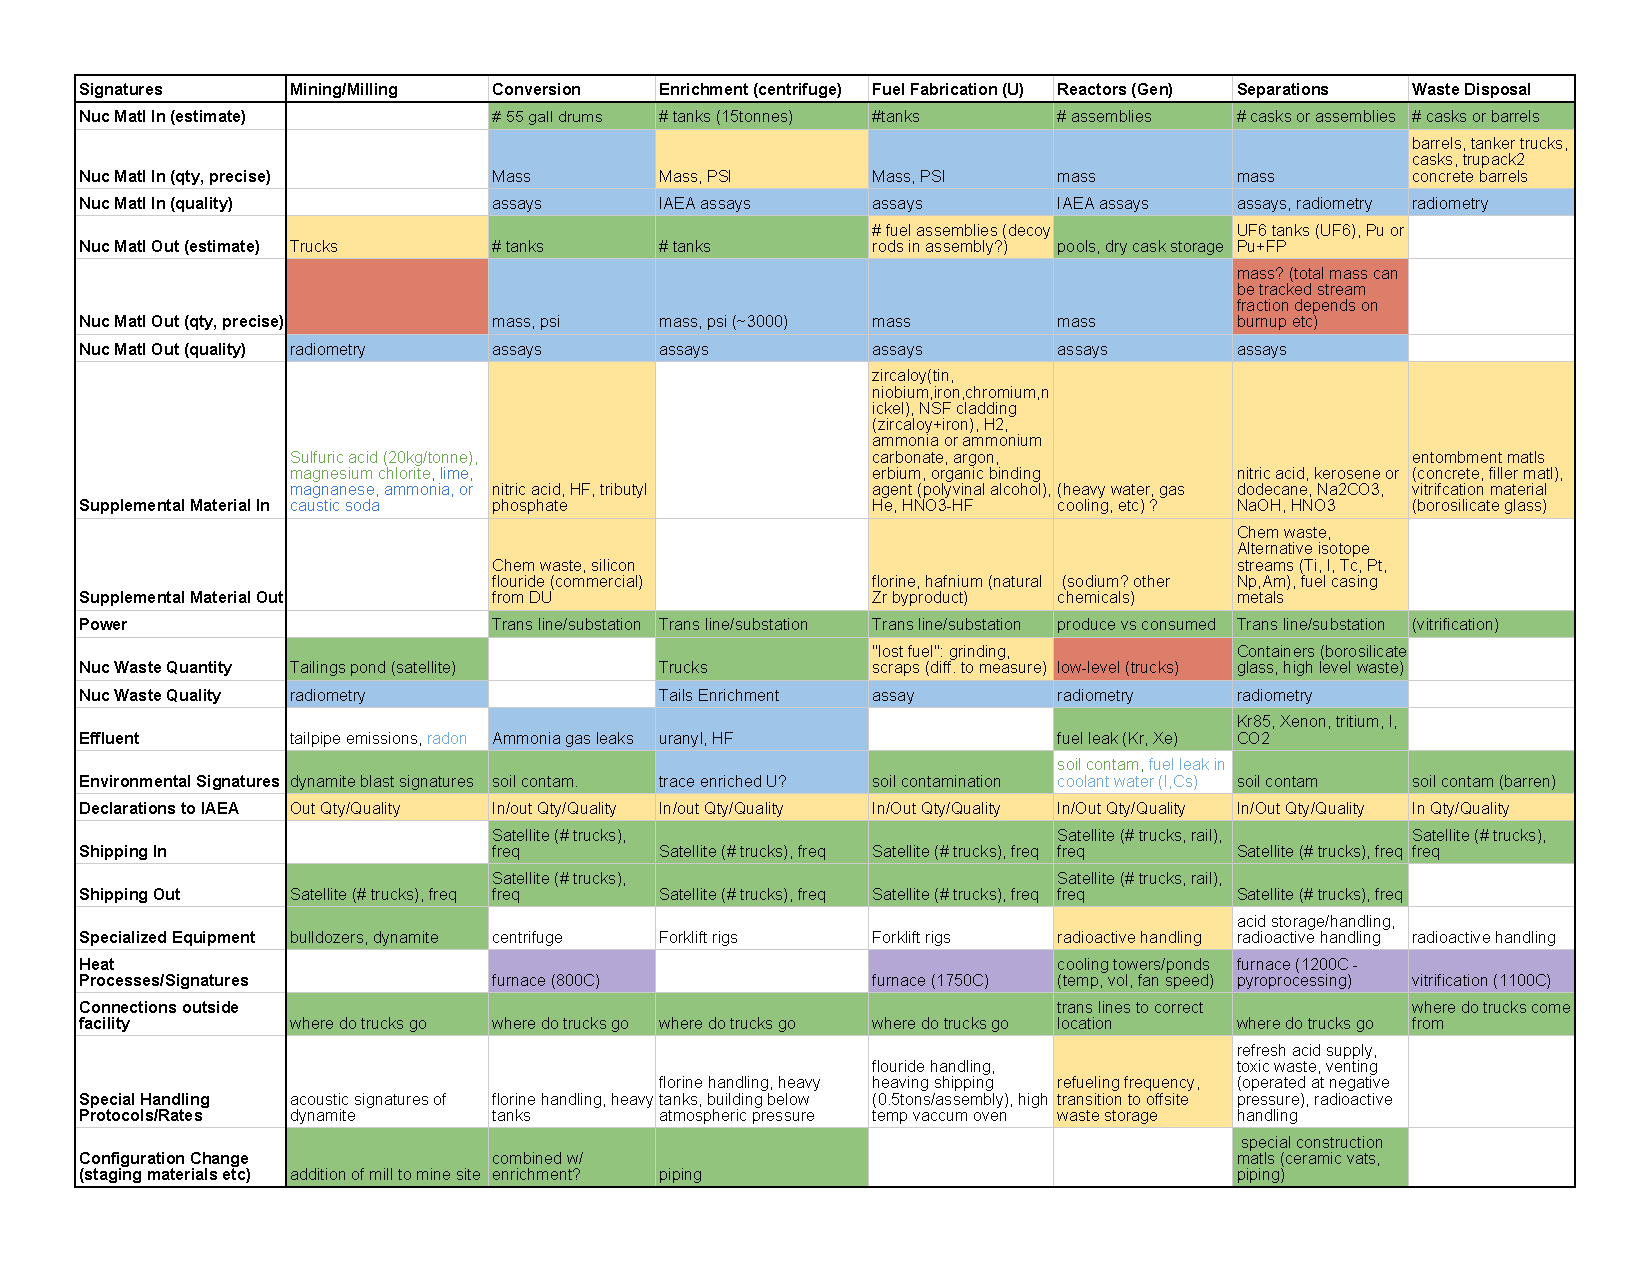
\includegraphics[scale=0.8]{./figs/signatures_table.pdf}
\end{center}
\caption{Table of potential signatures across the fuel cycle: measureable through open, independent sources such as satellite imagery (green), available through official inspections (blue), or potentially unreliable due to physical or political constraints (yellow).}
\label{fig:signatures}
\end{figure}

\Cyclus is being used to produce a variety of synthetic signals spanning a range of modalities that would be available either publicly or via official inspections (green or blue).  As detailed in Section \ref{s_results}, all facilities in \Cyclus inherently produce time-series data such as material flow, inventory, and \gls{SWU} consumption (for enrichment facilities). As seen in Figure \ref{fig:effluent}, \Cyclus can combine atmospheric transport models with facility effluent concentration ($I$) to track geographic dispersion. In this example, a simple atmospheric diffusion model of wind (from the left) is used to illustrate how a small clandestine reprocessing facility could be hidden in close proximity to two larger declared facilities\cite{hanna_handbook_1982}. 

% /Users/mbmcgarry/git/data_analysis/data/v1.3/pu_reprocess/
\begin{figure}%[htbp!]
\begin{center}
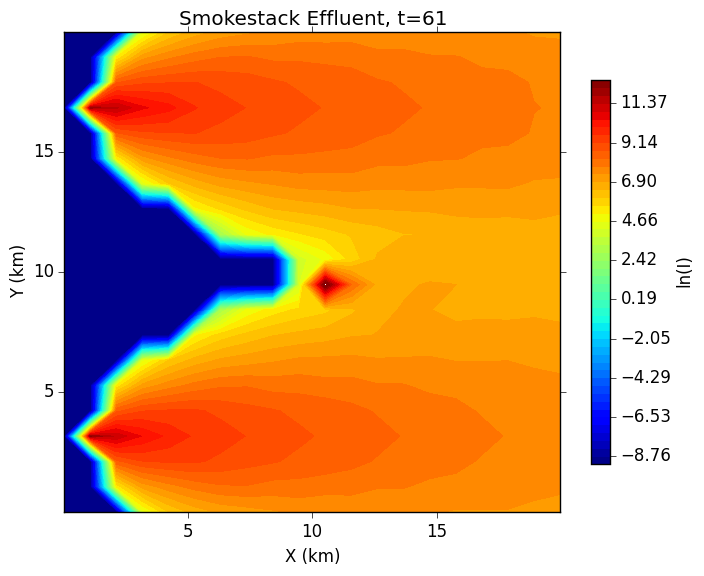
\includegraphics[natwidth=162bp,natheight=227bp, scale=0.4]{./figs/proper_diff_fr61.png}
\end{center}
\caption{Effluent transport with wind from left, hides a clandestine reprocessing facility x,y=(11,9) in close proximity to two declared facilities x,y=(1,3), (1,17)}
\label{fig:effluent}
\end{figure}

\Cyclus also models sparse, discrete-event data such as declared truck shipments or IAEA inspections that test for the presence of \gls{HEU}. Figure \ref{fig:inspect} pairs inspections with undeclared truck shipments of \gls{HEU}.  IAEA inspections typically involve multiple swipe samples per location, with some likelihood of false-positive or false-negative results\cite{ryjinski_idms_2003}. In this example, it is assumed that the likelihood of detecting \gls{HEU} in the enrichment facility increases with each shipment, because contamination is possible when \gls{HEU} is removed from cascades and bottled for shipping.  The undeclared \gls{HEU} shipments are shown as black bars, where amplitude incorporates the cumulative amount of \gls{HEU} that has been produced at the facility. The colored dots scale from yellow to red, indicating the fraction of positive swipes at an \gls{IAEA} inspector visit, assuming a total of 10 swipes are taken per inspection and a 30\% chance that an individual swipe may produce a false reading.  

% /Users/mbmcgarry/git/data_analysis/data/UM_data/multi_modal_v1.3/single_runs/inspect_example
\begin{figure}%[htbp!]
\begin{center}
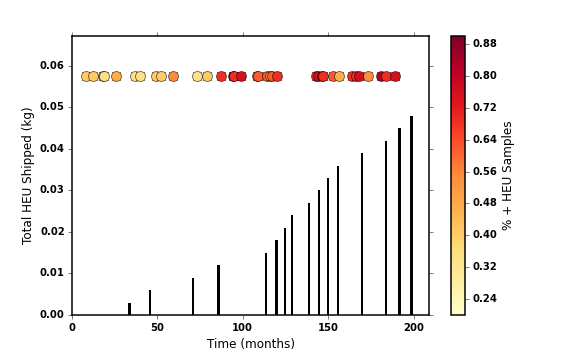
\includegraphics[natwidth=162bp,natheight=227bp, scale=0.6]{./figs/mm_5enrich_tinytails_inspinspect_ship.png}
\end{center}
\caption{Black bars indicate clandestine shipments of \gls{HEU}, amplitudes show gross \gls{HEU} production at the enrichment facility.  Colored circles are fraction of swipes (out of 10) testing positive for \gls{HEU} during an inspection. Both false positives and false negatives may be present, introducing uncertainty into the data.}
\label{fig:inspect}
\end{figure}

Figure \ref{fig:false_inspect} shows the breakdown of true positive, false positive, and false negative results for each inspection.  Before month 30, no \gls{HEU} has been produced in the facility, so any ``positive'' swipes are false-positives (tan). Once the facility begins producing \gls{HEU}, likelihood of contamination increases until it is detected near month 80. If the swipe tests were perfect, there would be a 100\% detection rate for all inspections after that time. However, the possibility of false-negatives (pink), make the measured inspection data appear to be the tan signal before month 80 and the red signal after month 80.  In this scenario, it would be difficult for an inspector to conclude that \gls{HEU} was being produced with this dataset alone.

\begin{figure}%[htbp!]
\begin{center}
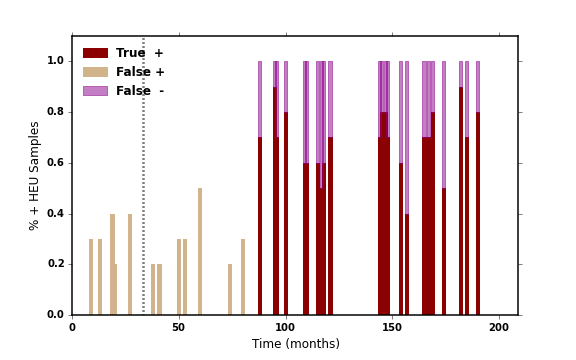
\includegraphics[natwidth=162bp,natheight=227bp, scale=0.6]{./figs/mm_5enrich_tinytails_inspswipe_rates.png}
\end{center}
\caption{The scenario in Figure \ref{fig:inspect} had a 30\% rate for both false-positives and false-negatives. Before month 30, no HEU has been produced so all detections are false positives (tan). Once \gls{HEU} contamination is present (near month 80), true detections (red) combine with false-negatives (pink), resulting in a effective 70\% detection rate.}
\label{fig:false_inspect}
\end{figure}
